\raggedbottom
 \setlength{\parskip}{0.5em}
\chapter{绪论}


\section{标题}
\subsection{副标题}

这是APA引用(\cite{pargament_apa_2013})。

如图\ref{fig1}所示,这是一张logo图。

\begin{figure}[!htb]
	\centering
	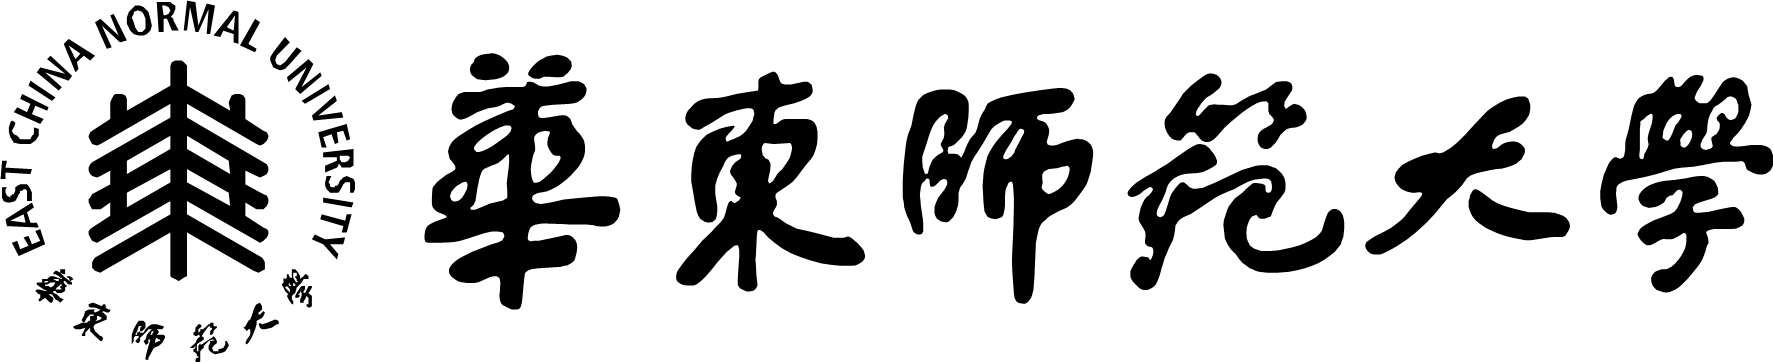
\includegraphics[width=3in]{1_figures/logo.png}
	\caption{标题}
	\label{fig1}
\end{figure}


这是表\ref{table_example}。
\begin{table}[!htb]
    \caption{三线表标题}
    \label{table_example}
    \centering
    \begin{tabular}{cccccc}
        \hline
        &	0 &	1	& 2 &	...&	n	\\
                \hline
0&	S(0)	&S(0)	&S(0)&	...	&S(0)	\\
1&	S(1)	&S(1)	&S(1)&	...	&S(1)	\\	
        \hline
    \end{tabular}
\end{table}

这是公式:
$$
v=\frac{s}{t}
$$
其中,$v$表示v我50,$s$表示购买力,$t$表示购买目标(target)。


这也是一个表,由于太长了,所以放到单独的文件中再进行导入。

% Please add the following required packages to your document preamble:
% \usepackage{booktabs}
% \usepackage{longtable}
% Note: It may be necessary to compile the document several times to get a multi-page table to line up properly
\begin{landscape}
\begin{longtable}[c]{@{}
    p{0.10\linewidth}
    p{0.10\linewidth}
    p{0.10\linewidth}
    p{0.10\linewidth}
    p{0.10\linewidth}
    p{0.10\linewidth}
    p{0.10\linewidth}
    p{0.10\linewidth}
@{}}
\caption{三线表样例2}
\label{tab:template2}\\
\toprule
1 & 2 & 3 & 4 & 1 & 2 & 3 & 4 \\* \midrule
\endfirsthead
%
\multicolumn{8}{c}%
{{\bfseries Table \thetable\ continued from previous page}} \\
\toprule
1 & 2 & 3 & 4 & 1 & 2 & 3 & 4 \\* \midrule
\endhead
%
\bottomrule
\endfoot
%
\endlastfoot
%
a  &  a & a  & a  &  a & a   & a  & a \\
a  &  a & a  & a  &  a & a   & a  & a \\
a  &  a & a  & a  &  a & a   & a  & a \\
a  &  a & a  & a  &  a & a   & a  & a \\
a  &  a & a  & a  &  a & a   & a  & a \\
a  &  a & a  & a  &  a & a   & a  & a \\* \bottomrule
\end{longtable}
\end{landscape}

